\question{Газовые лазеры. CO2-лазеры низкого давления}
Генерация осуществляется в импульсном и непрерывном режимах на 
колебательно-вращательных переходах в системе нижних колебательных уровней 
основного электронного состояния молекулы \( CO_2 \).
\begin{figure}[h]
    \center
    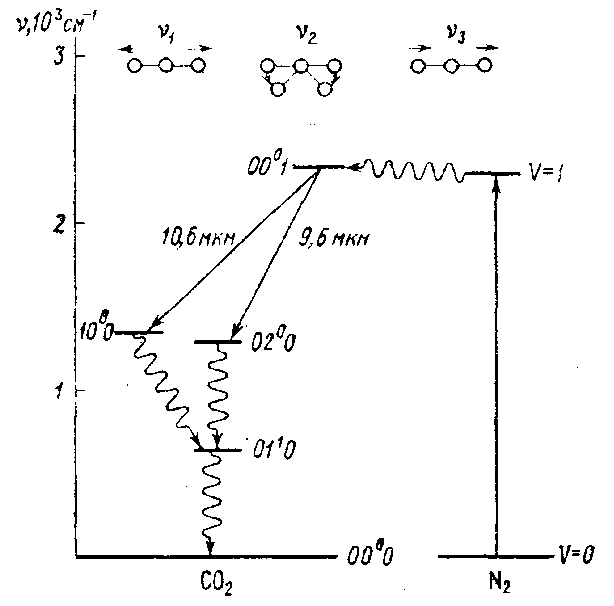
\includegraphics[width=.47\textwidth]{21}
    \caption{Уровни энергии молекулы \( CO_2 \)}
\end{figure}
Верхним лазерным уровнем является первое возбуждённое состояние несимметричного 
валентного колебания \( 001 \), нижними -- либо первое возбуждённое состояние 
симметричного валентного колебания \( 100\ (\lambda=10,6~\text{мкм}) \), либо 
второе возбуждённое состояние деформационного колебания 
\( 020\ (\lambda=9,6~\text{мкм}) \).

Инверсия создаётся в электрическом разряде при столкновениях с молекулами 
\( N_2 \), которые возбуждаются электронами разряда, а также при прямом 
возбуждении колебания \( 001 \) при столкновениях с электронами.

В наиболее распространённой рабочей смеси \( CO_2 \)-лазера \((CO_2:N_2:He)\) 
углекислый газ излучает, азот накапливает энергию, а гелий опустошает нижние 
лазерные уровни. Кроме того, гелий облегчает электрический разряд и охлаждает 
газовую смесь.

При низком давлении используется продольный разряд в относительно длинных 
газоразрядных трубках.

Для \( CO_2 \)-лазеров характерны большой КПД, высокие мощности и энергия 
непрерывного и импульсного режимов работы.